\section{Implementacja systemu na poziomie klas}
Oprogramowanie podzielono na sześć klas: \emph{App}, \emph{VideoCapture}, \emph{YoloInferenceConfig}, \emph{ImageProcessor}, \emph{VideoProcessingEngine} oraz \emph{GUI}.

\emph{App} jest punktem centralnym aplikacji. W tym miejscu rozpoczyna się program i tworzone są instancję pozostałych pięciu klas. Pierwszym zadaniem klasy jest uruchomienie wszystkich modułów w odpowiedniej kolejności. Następnie klasa ta służy jako interfejs do komunikacji między sekcją interfejsu graficznego (\emph{GUI}), a sekcją logiczną -- w tym do pobrania informacji o dostępnych kamerach (\emph{VideoCapture}), ustawienia danych detektora (\emph{ImageProcessor}) oraz obustronnej komunikacji z silnikiem przetwarzającym klatki wideo (\emph{VideoProcessingEngine}). 
Ponadto, klasa ta implementuje metodę, która uruchamia alarm dźwiękowy (\emph{{play\_audio\_alert}}). 

\emph{VideoCapture} służy do obługi źródła wideo. Klasa dostarcza kluczową metode, \emph{get\_frame}, której wywołanie zwraca informację o tym czy źródło wideo nadal jest dostępne oraz najnowszą dostępną klatkę z kamery. Ponadto warto wyróżnić metodę do pozyskania dostępnych do użycia kamer (\emph{get\_available\_sources}).

\emph{YoloInferenceConfig} jest to klasa, której głównym celem jest przechowywanie parametrów inferencji (progu ufności oraz wykrywanych klas) oraz dostarczenie metod do zmiany tych parametrów. Klase utworzono dla zachowania większej czytelności kodu w \emph{ImageProcessor}, dlatego też jest ona dziedziczona przez \emph{ImageProcessor} właśnie. W chwili uruchomienia aplikacji, klasa jest inicjalizowana domyślnymi parametrami: próg ufności równy $0.5$ oraz \emph{człowiek} jako wykrywany klasa. 

\emph{ImageProcessor} służy do manipulacji oraz analizy obrazu. Kluczowe dwie metody to \emph{detect\_objects}, zwracająca liczbe wykrytych obiektów oraz wyniki detekcji na podstawie podanej klatki obrazu, oraz \emph{visualize\_objects\_presence}, która na postawie w.w. wyników detekcji, rysuję prostokąty ograniczające dookoła wykrytych obiektów.

\emph{VideoProcessingEngine} stworzono w celu koordynacji i rozplanowania wszystkich zadań koniecznych do uzyskania kolejnych klatek obrazu, gotowych do wyświetlenia w graficzym interfejsie użytkownika, oraz realizacji celu alarmowania dźwiękowego użytkownika, kiedy jest to konieczne. Zbiór zadań zawiera pobranie klatki z kamery, detekcję obiektów, przetworzenie klatki w celu wizualizacji obiektów, alarmowanie dźwiękowe użytkownika oraz umieszczenie klatki w buforze wyjściowym. Zadania te nie mają implementacji w samej klasie i są metodami wywoływanymi z innych klas (\emph{App}, \emph{ImageProcessor} oraz \emph{VideoCapture}). Jest to najważniejszy element całego systemu, określający w stopniu znacznym jego architekturę, scalającym kluczowe komponenty oraz mającym główny wpływ na wydajność rozwiązania.

\emph{GUI} to graficzny interfejs użytkownika naszej aplikacji. Składa się on z wyświetlacza klatek obrazu oraz panelu sterowania. Tak jak to wcześniej wspomniano, używa on \emph{App} w celu komunikacji z resztą modułów. Tyczy się to zarówno komunikacji dwustronnej z \emph{ImageProcessor} oraz \emph{VideoCapture}, potrzebnej do panelu sterowania, oraz jednostronnej z \emph{VideoProcessingEngine} w celu pobrania klatki bufora wyjściowego.  

Opisane zależności komunikacyjne między klasami, w tym typy połączeń między nimi (kompozycja, agregacja, dziedziczenie) zilustrowano uprosczonym diagramem UML na rysunku \ref{fig:uprosczony-diagram-klas}. Pełen diagram UML przedstawiono na rysunku \ref{fig:diagram-klas}. 

\begin{figure}[H]
    \centering
    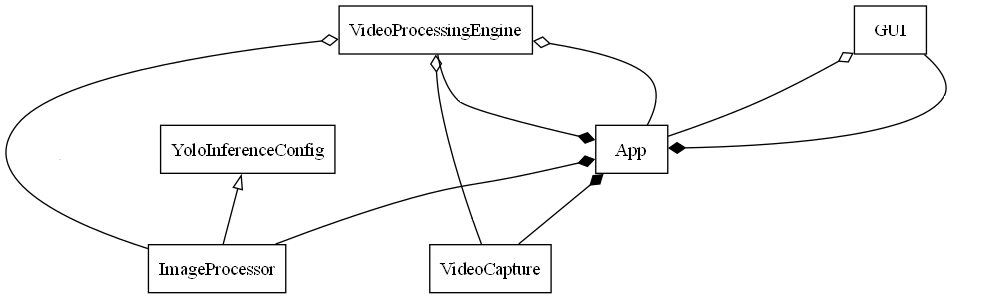
\includegraphics[width=\linewidth]{r_implementacja/klasy/simplified_classes.png}
    \caption{Uprosczony diagram klas UML (bez metod i pól) wygenerowany przez bilbiotekę \emph{pylint}.}
    \label{fig:uprosczony-diagram-klas}
\end{figure}

Tak jak wspomniano klasa \emph{YoloInferenceConfig} nie jest instancjowana -- programowe użycie jej pól odbywa się wewnątrz \emph{ImageProcessor}, zaś jej metody są wywoływane poprzez obiekt klasy \emph{ImageProcessor}. Jest to umożliwione dzięki dziedziczeniu \emph{YoloInferenceConfig} przez \emph{ImageProcessor}.

\emph{App} jako punkt startowy aplikacji tworzy w swoim konstruktorze obiekty klas \emph{VideoCapture}, \emph{ImageProcessor}, \emph{VideoProcessingEngine} oraz \emph{GUI} -- z perspektywy UML jest to agregacja tych klas. Nazwy tych obiektów to według kolejności: \emph{\_image\_processor}, \emph{\_video\_capture}, \emph{\_video\_processing\_engine} oraz \emph{\_gui}. Następnie, plik główny programu (\emph{main.py}) wywołuję metodę \emph{run}. Metoda ta uruchamia silnik generacji klatek (\emph{self.\_video\_processing\_engine.run()}) oraz wyświetla graficzny interfejs użytkownika \emph{self.\_gui.show()}. Po zamknięciu GUI wykonywana jest ostatnia istrukcja -- wyłączająca silnik generacji klatek (\emph{self.\_video\_processing\_engine.shutdown()}). Opisane użycie zareprezentowano fragmentem kodu w listingu \ref{lst:app-instancjowanie}.

\begin{lstlisting}[caption={Tworzenie obiektów klas wewnątrz \emph{App} oraz uruchomienie w niej różnych sekcji aplikacji.}, label={lst:app-instancjowanie}]
class App:
    # Konstruktor App
    def __init__(self) -> None:
        # ... reszta kodu
        # Tworzenie obiektow klas:
        self._video_capture = VideoCapture()
        self._image_processor = ImageProcessor()
        self._video_processing_engine = VideoProcessingEngine(self._video_capture, self._image_processor, self)
        self._gui = GUI(self)
        # reszta kodu ...

    # Metoda uruchamiajaca poszczegolne sekcje aplikacji
    def run(self) -> None:
        self._video_processing_engine.run()
        self._gui.show()
        self._video_processing_engine.shutdown()
\end{lstlisting}





\begin{figure}[H]
    \centering
    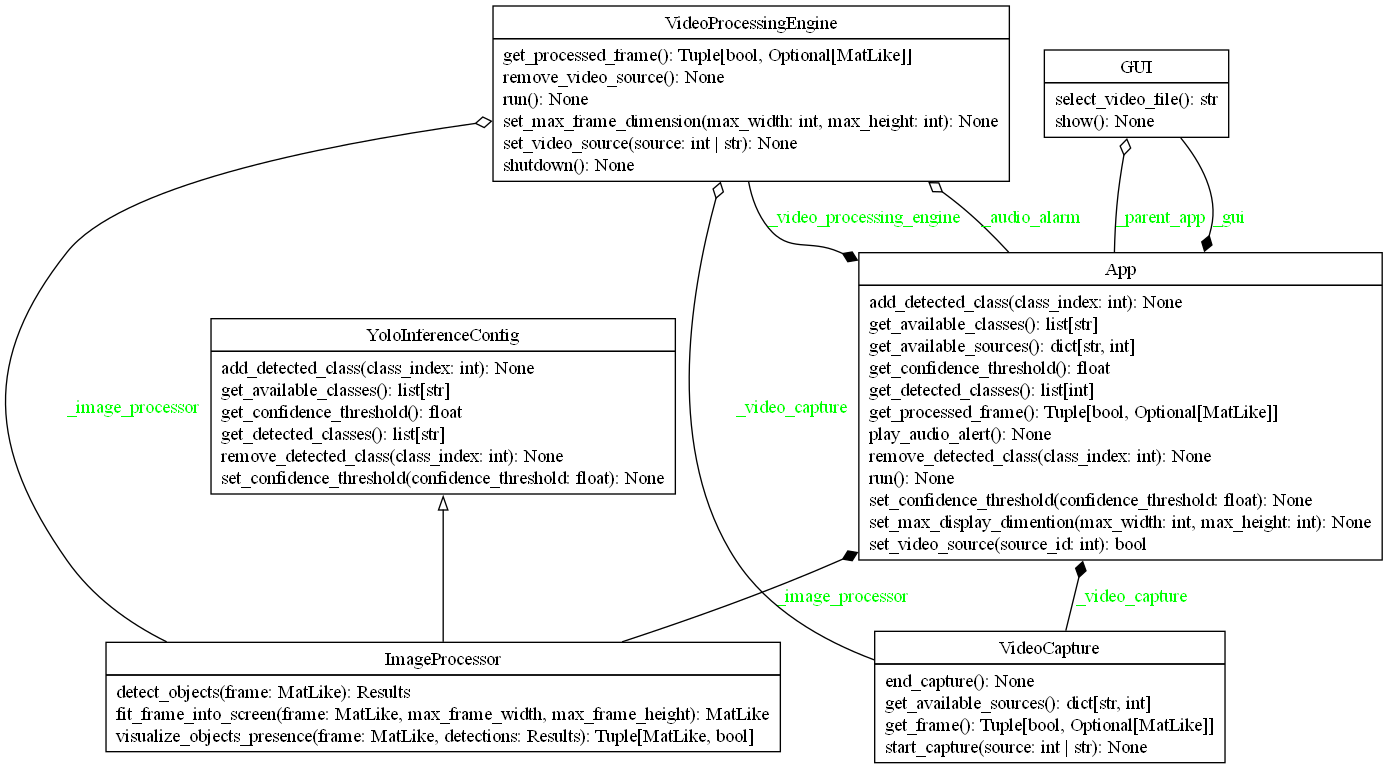
\includegraphics[angle=270, scale = 0.85]{r_implementacja/klasy/classes_MyProject.png}
    \caption{Diagram klas UML wygenerowany przez bilbiotekę \emph{pylint}.}
    \label{fig:diagram-klas}
\end{figure}